% Created by tikzDevice version 0.12 on 2019-04-10 00:22:01
% !TEX encoding = UTF-8 Unicode
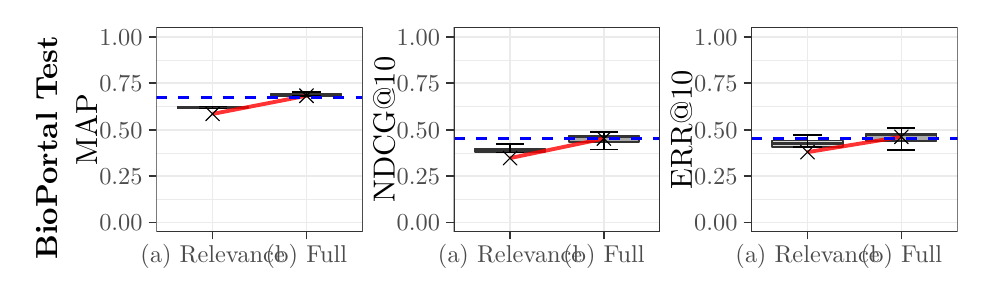
\begin{tikzpicture}[x=1pt,y=1pt]
\definecolor{fillColor}{RGB}{255,255,255}
\path[use as bounding box,fill=fillColor,fill opacity=0.00] (0,0) rectangle (336.06, 86.72);
\begin{scope}
\path[clip] ( 13.61,  0.00) rectangle (121.09, 86.72);
\definecolor{drawColor}{RGB}{255,255,255}
\definecolor{fillColor}{RGB}{255,255,255}

\path[draw=drawColor,line width= 0.6pt,line join=round,line cap=round,fill=fillColor] ( 13.61,  0.00) rectangle (121.09, 86.72);
\end{scope}
\begin{scope}
\path[clip] ( 46.47, 12.95) rectangle (121.09, 86.72);
\definecolor{fillColor}{RGB}{255,255,255}

\path[fill=fillColor] ( 46.47, 12.95) rectangle (121.09, 86.72);
\definecolor{drawColor}{gray}{0.92}

\path[draw=drawColor,line width= 0.3pt,line join=round] ( 46.47, 24.69) --
	(121.09, 24.69);

\path[draw=drawColor,line width= 0.3pt,line join=round] ( 46.47, 41.46) --
	(121.09, 41.46);

\path[draw=drawColor,line width= 0.3pt,line join=round] ( 46.47, 58.22) --
	(121.09, 58.22);

\path[draw=drawColor,line width= 0.3pt,line join=round] ( 46.47, 74.99) --
	(121.09, 74.99);

\path[draw=drawColor,line width= 0.6pt,line join=round] ( 46.47, 16.31) --
	(121.09, 16.31);

\path[draw=drawColor,line width= 0.6pt,line join=round] ( 46.47, 33.07) --
	(121.09, 33.07);

\path[draw=drawColor,line width= 0.6pt,line join=round] ( 46.47, 49.84) --
	(121.09, 49.84);

\path[draw=drawColor,line width= 0.6pt,line join=round] ( 46.47, 66.61) --
	(121.09, 66.61);

\path[draw=drawColor,line width= 0.6pt,line join=round] ( 46.47, 83.37) --
	(121.09, 83.37);

\path[draw=drawColor,line width= 0.6pt,line join=round] ( 66.83, 12.95) --
	( 66.83, 86.72);

\path[draw=drawColor,line width= 0.6pt,line join=round] (100.74, 12.95) --
	(100.74, 86.72);

\path[] ( 64.86, 57.18) -- ( 68.79, 61.10);

\path[] ( 64.86, 61.10) -- ( 68.79, 57.18);

\path[] ( 64.86, 57.45) -- ( 68.79, 61.38);

\path[] ( 64.86, 61.38) -- ( 68.79, 57.45);

\path[] ( 64.86, 35.95) -- ( 68.79, 39.88);

\path[] ( 64.86, 39.88) -- ( 68.79, 35.95);

\path[] ( 64.86, 49.28) -- ( 68.79, 53.20);

\path[] ( 64.86, 53.20) -- ( 68.79, 49.28);
\definecolor{drawColor}{gray}{0.20}

\path[draw=drawColor,line width= 0.6pt,line join=round] ( 66.83, 58.21) -- ( 66.83, 58.24);

\path[draw=drawColor,line width= 0.6pt,line join=round] ( 66.83, 57.64) -- ( 66.83, 57.54);
\definecolor{fillColor}{RGB}{220,220,220}

\path[draw=drawColor,line width= 0.6pt,line join=round,line cap=round,fill=fillColor] ( 54.11, 58.21) --
	( 54.11, 57.64) --
	( 79.54, 57.64) --
	( 79.54, 58.21) --
	( 54.11, 58.21) --
	cycle;

\path[draw=drawColor,line width= 1.1pt,line join=round] ( 54.11, 58.01) -- ( 79.54, 58.01);

\path[] ( 98.78, 56.79) -- (102.71, 60.71);

\path[] ( 98.78, 60.71) -- (102.71, 56.79);

\path[draw=drawColor,line width= 0.6pt,line join=round] (100.74, 62.90) -- (100.74, 63.37);

\path[draw=drawColor,line width= 0.6pt,line join=round] (100.74, 61.99) -- (100.74, 61.91);
\definecolor{fillColor}{RGB}{169,169,169}

\path[draw=drawColor,line width= 0.6pt,line join=round,line cap=round,fill=fillColor] ( 88.02, 62.90) --
	( 88.02, 61.99) --
	(113.46, 61.99) --
	(113.46, 62.90) --
	( 88.02, 62.90) --
	cycle;

\path[draw=drawColor,line width= 1.1pt,line join=round] ( 88.02, 62.25) -- (113.46, 62.25);
\definecolor{drawColor}{RGB}{255,0,0}

\path[draw=drawColor,draw opacity=0.80,line width= 1.4pt,line join=round] ( 66.83, 55.55) --
	(100.74, 62.12);
\definecolor{drawColor}{RGB}{0,0,0}

\path[draw=drawColor,line width= 0.4pt,line join=round,line cap=round] ( 64.33, 53.06) -- ( 69.32, 58.05);

\path[draw=drawColor,line width= 0.4pt,line join=round,line cap=round] ( 64.33, 58.05) -- ( 69.32, 53.06);

\path[draw=drawColor,line width= 0.4pt,line join=round,line cap=round] ( 98.25, 59.62) -- (103.24, 64.62);

\path[draw=drawColor,line width= 0.4pt,line join=round,line cap=round] ( 98.25, 64.62) -- (103.24, 59.62);

\path[draw=drawColor,line width= 0.6pt,line join=round] ( 61.74, 58.24) --
	( 71.91, 58.24);

\path[draw=drawColor,line width= 0.6pt,line join=round] ( 66.83, 58.24) --
	( 66.83, 57.54);

\path[draw=drawColor,line width= 0.6pt,line join=round] ( 61.74, 57.54) --
	( 71.91, 57.54);

\path[draw=drawColor,line width= 0.6pt,line join=round] ( 95.66, 63.37) --
	(105.83, 63.37);

\path[draw=drawColor,line width= 0.6pt,line join=round] (100.74, 63.37) --
	(100.74, 61.91);

\path[draw=drawColor,line width= 0.6pt,line join=round] ( 95.66, 61.91) --
	(105.83, 61.91);
\definecolor{drawColor}{RGB}{0,0,255}

\path[draw=drawColor,line width= 1.1pt,dash pattern=on 4pt off 4pt ,line join=round] ( 46.47, 61.61) -- (121.09, 61.61);
\definecolor{drawColor}{gray}{0.20}

\path[draw=drawColor,line width= 0.6pt,line join=round,line cap=round] ( 46.47, 12.95) rectangle (121.09, 86.72);
\end{scope}
\begin{scope}
\path[clip] (  0.00,  0.00) rectangle (336.06, 86.72);
\definecolor{drawColor}{gray}{0.30}

\node[text=drawColor,anchor=base east,inner sep=0pt, outer sep=0pt, scale=  0.88] at ( 41.52, 13.28) {0.00};

\node[text=drawColor,anchor=base east,inner sep=0pt, outer sep=0pt, scale=  0.88] at ( 41.52, 30.04) {0.25};

\node[text=drawColor,anchor=base east,inner sep=0pt, outer sep=0pt, scale=  0.88] at ( 41.52, 46.81) {0.50};

\node[text=drawColor,anchor=base east,inner sep=0pt, outer sep=0pt, scale=  0.88] at ( 41.52, 63.57) {0.75};

\node[text=drawColor,anchor=base east,inner sep=0pt, outer sep=0pt, scale=  0.88] at ( 41.52, 80.34) {1.00};
\end{scope}
\begin{scope}
\path[clip] (  0.00,  0.00) rectangle (336.06, 86.72);
\definecolor{drawColor}{gray}{0.20}

\path[draw=drawColor,line width= 0.6pt,line join=round] ( 43.72, 16.31) --
	( 46.47, 16.31);

\path[draw=drawColor,line width= 0.6pt,line join=round] ( 43.72, 33.07) --
	( 46.47, 33.07);

\path[draw=drawColor,line width= 0.6pt,line join=round] ( 43.72, 49.84) --
	( 46.47, 49.84);

\path[draw=drawColor,line width= 0.6pt,line join=round] ( 43.72, 66.61) --
	( 46.47, 66.61);

\path[draw=drawColor,line width= 0.6pt,line join=round] ( 43.72, 83.37) --
	( 46.47, 83.37);
\end{scope}
\begin{scope}
\path[clip] (  0.00,  0.00) rectangle (336.06, 86.72);
\definecolor{drawColor}{gray}{0.20}

\path[draw=drawColor,line width= 0.6pt,line join=round] ( 66.83, 10.20) --
	( 66.83, 12.95);

\path[draw=drawColor,line width= 0.6pt,line join=round] (100.74, 10.20) --
	(100.74, 12.95);
\end{scope}
\begin{scope}
\path[clip] (  0.00,  0.00) rectangle (336.06, 86.72);
\definecolor{drawColor}{gray}{0.30}

\node[text=drawColor,anchor=base,inner sep=0pt, outer sep=0pt, scale=  0.88] at ( 66.83,  1.94) {(a) Relevance};

\node[text=drawColor,anchor=base,inner sep=0pt, outer sep=0pt, scale=  0.88] at (100.74,  1.94) {(b) Full};
\end{scope}
\begin{scope}
\path[clip] (  0.00,  0.00) rectangle (336.06, 86.72);
\definecolor{drawColor}{RGB}{0,0,0}

\node[text=drawColor,rotate= 90.00,anchor=base,inner sep=0pt, outer sep=0pt, scale=  1.10] at ( 25.08, 49.84) {MAP};
\end{scope}
\begin{scope}
\path[clip] (121.09,  0.00) rectangle (228.57, 86.72);
\definecolor{drawColor}{RGB}{255,255,255}
\definecolor{fillColor}{RGB}{255,255,255}

\path[draw=drawColor,line width= 0.6pt,line join=round,line cap=round,fill=fillColor] (121.09,  0.00) rectangle (228.57, 86.72);
\end{scope}
\begin{scope}
\path[clip] (153.95, 12.95) rectangle (228.57, 86.72);
\definecolor{fillColor}{RGB}{255,255,255}

\path[fill=fillColor] (153.95, 12.95) rectangle (228.57, 86.72);
\definecolor{drawColor}{gray}{0.92}

\path[draw=drawColor,line width= 0.3pt,line join=round] (153.95, 24.69) --
	(228.57, 24.69);

\path[draw=drawColor,line width= 0.3pt,line join=round] (153.95, 41.46) --
	(228.57, 41.46);

\path[draw=drawColor,line width= 0.3pt,line join=round] (153.95, 58.22) --
	(228.57, 58.22);

\path[draw=drawColor,line width= 0.3pt,line join=round] (153.95, 74.99) --
	(228.57, 74.99);

\path[draw=drawColor,line width= 0.6pt,line join=round] (153.95, 16.31) --
	(228.57, 16.31);

\path[draw=drawColor,line width= 0.6pt,line join=round] (153.95, 33.07) --
	(228.57, 33.07);

\path[draw=drawColor,line width= 0.6pt,line join=round] (153.95, 49.84) --
	(228.57, 49.84);

\path[draw=drawColor,line width= 0.6pt,line join=round] (153.95, 66.61) --
	(228.57, 66.61);

\path[draw=drawColor,line width= 0.6pt,line join=round] (153.95, 83.37) --
	(228.57, 83.37);

\path[draw=drawColor,line width= 0.6pt,line join=round] (174.31, 12.95) --
	(174.31, 86.72);

\path[draw=drawColor,line width= 0.6pt,line join=round] (208.22, 12.95) --
	(208.22, 86.72);

\path[] (172.34, 14.67) -- (176.27, 18.60);

\path[] (172.34, 18.60) -- (176.27, 14.67);

\path[] (172.34, 32.93) -- (176.27, 36.85);

\path[] (172.34, 36.85) -- (176.27, 32.93);
\definecolor{drawColor}{gray}{0.20}

\path[draw=drawColor,line width= 0.6pt,line join=round] (174.31, 43.11) -- (174.31, 44.73);

\path[draw=drawColor,line width= 0.6pt,line join=round] (174.31, 41.81) -- (174.31, 41.62);
\definecolor{fillColor}{RGB}{220,220,220}

\path[draw=drawColor,line width= 0.6pt,line join=round,line cap=round,fill=fillColor] (161.59, 43.11) --
	(161.59, 41.81) --
	(187.03, 41.81) --
	(187.03, 43.11) --
	(161.59, 43.11) --
	cycle;

\path[draw=drawColor,line width= 1.1pt,line join=round] (161.59, 42.62) -- (187.03, 42.62);

\path[draw=drawColor,line width= 0.6pt,line join=round] (208.22, 47.72) -- (208.22, 49.01);

\path[draw=drawColor,line width= 0.6pt,line join=round] (208.22, 45.36) -- (208.22, 42.69);
\definecolor{fillColor}{RGB}{169,169,169}

\path[draw=drawColor,line width= 0.6pt,line join=round,line cap=round,fill=fillColor] (195.50, 47.72) --
	(195.50, 45.36) --
	(220.94, 45.36) --
	(220.94, 47.72) --
	(195.50, 47.72) --
	cycle;

\path[draw=drawColor,line width= 1.1pt,line join=round] (195.50, 47.26) -- (220.94, 47.26);
\definecolor{drawColor}{RGB}{255,0,0}

\path[draw=drawColor,draw opacity=0.80,line width= 1.4pt,line join=round] (174.31, 39.59) --
	(208.22, 46.65);
\definecolor{drawColor}{RGB}{0,0,0}

\path[draw=drawColor,line width= 0.4pt,line join=round,line cap=round] (171.81, 37.09) -- (176.80, 42.09);

\path[draw=drawColor,line width= 0.4pt,line join=round,line cap=round] (171.81, 42.09) -- (176.80, 37.09);

\path[draw=drawColor,line width= 0.4pt,line join=round,line cap=round] (205.73, 44.15) -- (210.72, 49.15);

\path[draw=drawColor,line width= 0.4pt,line join=round,line cap=round] (205.73, 49.15) -- (210.72, 44.15);

\path[draw=drawColor,line width= 0.6pt,line join=round] (169.22, 44.73) --
	(179.39, 44.73);

\path[draw=drawColor,line width= 0.6pt,line join=round] (174.31, 44.73) --
	(174.31, 41.62);

\path[draw=drawColor,line width= 0.6pt,line join=round] (169.22, 41.62) --
	(179.39, 41.62);

\path[draw=drawColor,line width= 0.6pt,line join=round] (203.14, 49.01) --
	(213.31, 49.01);

\path[draw=drawColor,line width= 0.6pt,line join=round] (208.22, 49.01) --
	(208.22, 42.69);

\path[draw=drawColor,line width= 0.6pt,line join=round] (203.14, 42.69) --
	(213.31, 42.69);
\definecolor{drawColor}{RGB}{0,0,255}

\path[draw=drawColor,line width= 1.1pt,dash pattern=on 4pt off 4pt ,line join=round] (153.95, 46.64) -- (228.57, 46.64);
\definecolor{drawColor}{gray}{0.20}

\path[draw=drawColor,line width= 0.6pt,line join=round,line cap=round] (153.95, 12.95) rectangle (228.57, 86.72);
\end{scope}
\begin{scope}
\path[clip] (  0.00,  0.00) rectangle (336.06, 86.72);
\definecolor{drawColor}{gray}{0.30}

\node[text=drawColor,anchor=base east,inner sep=0pt, outer sep=0pt, scale=  0.88] at (149.00, 13.28) {0.00};

\node[text=drawColor,anchor=base east,inner sep=0pt, outer sep=0pt, scale=  0.88] at (149.00, 30.04) {0.25};

\node[text=drawColor,anchor=base east,inner sep=0pt, outer sep=0pt, scale=  0.88] at (149.00, 46.81) {0.50};

\node[text=drawColor,anchor=base east,inner sep=0pt, outer sep=0pt, scale=  0.88] at (149.00, 63.57) {0.75};

\node[text=drawColor,anchor=base east,inner sep=0pt, outer sep=0pt, scale=  0.88] at (149.00, 80.34) {1.00};
\end{scope}
\begin{scope}
\path[clip] (  0.00,  0.00) rectangle (336.06, 86.72);
\definecolor{drawColor}{gray}{0.20}

\path[draw=drawColor,line width= 0.6pt,line join=round] (151.20, 16.31) --
	(153.95, 16.31);

\path[draw=drawColor,line width= 0.6pt,line join=round] (151.20, 33.07) --
	(153.95, 33.07);

\path[draw=drawColor,line width= 0.6pt,line join=round] (151.20, 49.84) --
	(153.95, 49.84);

\path[draw=drawColor,line width= 0.6pt,line join=round] (151.20, 66.61) --
	(153.95, 66.61);

\path[draw=drawColor,line width= 0.6pt,line join=round] (151.20, 83.37) --
	(153.95, 83.37);
\end{scope}
\begin{scope}
\path[clip] (  0.00,  0.00) rectangle (336.06, 86.72);
\definecolor{drawColor}{gray}{0.20}

\path[draw=drawColor,line width= 0.6pt,line join=round] (174.31, 10.20) --
	(174.31, 12.95);

\path[draw=drawColor,line width= 0.6pt,line join=round] (208.22, 10.20) --
	(208.22, 12.95);
\end{scope}
\begin{scope}
\path[clip] (  0.00,  0.00) rectangle (336.06, 86.72);
\definecolor{drawColor}{gray}{0.30}

\node[text=drawColor,anchor=base,inner sep=0pt, outer sep=0pt, scale=  0.88] at (174.31,  1.94) {(a) Relevance};

\node[text=drawColor,anchor=base,inner sep=0pt, outer sep=0pt, scale=  0.88] at (208.22,  1.94) {(b) Full};
\end{scope}
\begin{scope}
\path[clip] (  0.00,  0.00) rectangle (336.06, 86.72);
\definecolor{drawColor}{RGB}{0,0,0}

\node[text=drawColor,rotate= 90.00,anchor=base,inner sep=0pt, outer sep=0pt, scale=  1.10] at (132.56, 49.84) {NDCG@10};
\end{scope}
\begin{scope}
\path[clip] (228.57,  0.00) rectangle (336.06, 86.72);
\definecolor{drawColor}{RGB}{255,255,255}
\definecolor{fillColor}{RGB}{255,255,255}

\path[draw=drawColor,line width= 0.6pt,line join=round,line cap=round,fill=fillColor] (228.57,  0.00) rectangle (336.06, 86.72);
\end{scope}
\begin{scope}
\path[clip] (261.44, 12.95) rectangle (336.06, 86.72);
\definecolor{fillColor}{RGB}{255,255,255}

\path[fill=fillColor] (261.44, 12.95) rectangle (336.06, 86.72);
\definecolor{drawColor}{gray}{0.92}

\path[draw=drawColor,line width= 0.3pt,line join=round] (261.44, 24.69) --
	(336.06, 24.69);

\path[draw=drawColor,line width= 0.3pt,line join=round] (261.44, 41.46) --
	(336.06, 41.46);

\path[draw=drawColor,line width= 0.3pt,line join=round] (261.44, 58.22) --
	(336.06, 58.22);

\path[draw=drawColor,line width= 0.3pt,line join=round] (261.44, 74.99) --
	(336.06, 74.99);

\path[draw=drawColor,line width= 0.6pt,line join=round] (261.44, 16.31) --
	(336.06, 16.31);

\path[draw=drawColor,line width= 0.6pt,line join=round] (261.44, 33.07) --
	(336.06, 33.07);

\path[draw=drawColor,line width= 0.6pt,line join=round] (261.44, 49.84) --
	(336.06, 49.84);

\path[draw=drawColor,line width= 0.6pt,line join=round] (261.44, 66.61) --
	(336.06, 66.61);

\path[draw=drawColor,line width= 0.6pt,line join=round] (261.44, 83.37) --
	(336.06, 83.37);

\path[draw=drawColor,line width= 0.6pt,line join=round] (281.79, 12.95) --
	(281.79, 86.72);

\path[draw=drawColor,line width= 0.6pt,line join=round] (315.70, 12.95) --
	(315.70, 86.72);

\path[] (279.82, 14.57) -- (283.75, 18.50);

\path[] (279.82, 18.50) -- (283.75, 14.57);

\path[] (279.82, 36.04) -- (283.75, 39.96);

\path[] (279.82, 39.96) -- (283.75, 36.04);
\definecolor{drawColor}{gray}{0.20}

\path[draw=drawColor,line width= 0.6pt,line join=round] (281.79, 45.92) -- (281.79, 47.93);

\path[draw=drawColor,line width= 0.6pt,line join=round] (281.79, 43.52) -- (281.79, 43.50);
\definecolor{fillColor}{RGB}{220,220,220}

\path[draw=drawColor,line width= 0.6pt,line join=round,line cap=round,fill=fillColor] (269.07, 45.92) --
	(269.07, 43.52) --
	(294.51, 43.52) --
	(294.51, 45.92) --
	(269.07, 45.92) --
	cycle;

\path[draw=drawColor,line width= 1.1pt,line join=round] (269.07, 44.71) -- (294.51, 44.71);

\path[draw=drawColor,line width= 0.6pt,line join=round] (315.70, 48.47) -- (315.70, 50.46);

\path[draw=drawColor,line width= 0.6pt,line join=round] (315.70, 45.87) -- (315.70, 42.40);
\definecolor{fillColor}{RGB}{169,169,169}

\path[draw=drawColor,line width= 0.6pt,line join=round,line cap=round,fill=fillColor] (302.99, 48.47) --
	(302.99, 45.87) --
	(328.42, 45.87) --
	(328.42, 48.47) --
	(302.99, 48.47) --
	cycle;

\path[draw=drawColor,line width= 1.1pt,line join=round] (302.99, 48.16) -- (328.42, 48.16);
\definecolor{drawColor}{RGB}{255,0,0}

\path[draw=drawColor,draw opacity=0.80,line width= 1.4pt,line join=round] (281.79, 41.75) --
	(315.70, 47.27);
\definecolor{drawColor}{RGB}{0,0,0}

\path[draw=drawColor,line width= 0.4pt,line join=round,line cap=round] (279.29, 39.25) -- (284.28, 44.25);

\path[draw=drawColor,line width= 0.4pt,line join=round,line cap=round] (279.29, 44.25) -- (284.28, 39.25);

\path[draw=drawColor,line width= 0.4pt,line join=round,line cap=round] (313.21, 44.77) -- (318.20, 49.77);

\path[draw=drawColor,line width= 0.4pt,line join=round,line cap=round] (313.21, 49.77) -- (318.20, 44.77);

\path[draw=drawColor,line width= 0.6pt,line join=round] (276.70, 47.93) --
	(286.87, 47.93);

\path[draw=drawColor,line width= 0.6pt,line join=round] (281.79, 47.93) --
	(281.79, 43.50);

\path[draw=drawColor,line width= 0.6pt,line join=round] (276.70, 43.50) --
	(286.87, 43.50);

\path[draw=drawColor,line width= 0.6pt,line join=round] (310.62, 50.46) --
	(320.79, 50.46);

\path[draw=drawColor,line width= 0.6pt,line join=round] (315.70, 50.46) --
	(315.70, 42.40);

\path[draw=drawColor,line width= 0.6pt,line join=round] (310.62, 42.40) --
	(320.79, 42.40);
\definecolor{drawColor}{RGB}{0,0,255}

\path[draw=drawColor,line width= 1.1pt,dash pattern=on 4pt off 4pt ,line join=round] (261.44, 46.60) -- (336.06, 46.60);
\definecolor{drawColor}{gray}{0.20}

\path[draw=drawColor,line width= 0.6pt,line join=round,line cap=round] (261.44, 12.95) rectangle (336.06, 86.72);
\end{scope}
\begin{scope}
\path[clip] (  0.00,  0.00) rectangle (336.06, 86.72);
\definecolor{drawColor}{gray}{0.30}

\node[text=drawColor,anchor=base east,inner sep=0pt, outer sep=0pt, scale=  0.88] at (256.49, 13.28) {0.00};

\node[text=drawColor,anchor=base east,inner sep=0pt, outer sep=0pt, scale=  0.88] at (256.49, 30.04) {0.25};

\node[text=drawColor,anchor=base east,inner sep=0pt, outer sep=0pt, scale=  0.88] at (256.49, 46.81) {0.50};

\node[text=drawColor,anchor=base east,inner sep=0pt, outer sep=0pt, scale=  0.88] at (256.49, 63.57) {0.75};

\node[text=drawColor,anchor=base east,inner sep=0pt, outer sep=0pt, scale=  0.88] at (256.49, 80.34) {1.00};
\end{scope}
\begin{scope}
\path[clip] (  0.00,  0.00) rectangle (336.06, 86.72);
\definecolor{drawColor}{gray}{0.20}

\path[draw=drawColor,line width= 0.6pt,line join=round] (258.69, 16.31) --
	(261.44, 16.31);

\path[draw=drawColor,line width= 0.6pt,line join=round] (258.69, 33.07) --
	(261.44, 33.07);

\path[draw=drawColor,line width= 0.6pt,line join=round] (258.69, 49.84) --
	(261.44, 49.84);

\path[draw=drawColor,line width= 0.6pt,line join=round] (258.69, 66.61) --
	(261.44, 66.61);

\path[draw=drawColor,line width= 0.6pt,line join=round] (258.69, 83.37) --
	(261.44, 83.37);
\end{scope}
\begin{scope}
\path[clip] (  0.00,  0.00) rectangle (336.06, 86.72);
\definecolor{drawColor}{gray}{0.20}

\path[draw=drawColor,line width= 0.6pt,line join=round] (281.79, 10.20) --
	(281.79, 12.95);

\path[draw=drawColor,line width= 0.6pt,line join=round] (315.70, 10.20) --
	(315.70, 12.95);
\end{scope}
\begin{scope}
\path[clip] (  0.00,  0.00) rectangle (336.06, 86.72);
\definecolor{drawColor}{gray}{0.30}

\node[text=drawColor,anchor=base,inner sep=0pt, outer sep=0pt, scale=  0.88] at (281.79,  1.94) {(a) Relevance};

\node[text=drawColor,anchor=base,inner sep=0pt, outer sep=0pt, scale=  0.88] at (315.70,  1.94) {(b) Full};
\end{scope}
\begin{scope}
\path[clip] (  0.00,  0.00) rectangle (336.06, 86.72);
\definecolor{drawColor}{RGB}{0,0,0}

\node[text=drawColor,rotate= 90.00,anchor=base,inner sep=0pt, outer sep=0pt, scale=  1.10] at (240.04, 49.84) {ERR@10};
\end{scope}
\begin{scope}
\path[clip] (  0.00,  0.00) rectangle (336.06, 86.72);
\definecolor{drawColor}{RGB}{0,0,0}

\node[text=drawColor,rotate= 90.00,anchor=base,inner sep=0pt, outer sep=0pt, scale=  1.10] at ( 10.60, 43.36) {\bfseries BioPortal Test};
\end{scope}
\end{tikzpicture}
